\chapter[%
    Algorithms for Linear-Response Density Cumulant Theory
]{%
    Algorithms for Linear-Response Density Cumulant Theory
}
\label{ch:davidson}

\cref{ch:response} presented the LR-ODC-12 model for electronic excited states,
where excitation energies and transition properties are computed by
diagonalizing the parameter Hessian of the ODC-12 energy functional, with
respect to a metric that arises from the time-dependence of the parameter
responses.
Since number of parameters in the ODC-12 model scales as
\(
    \mathcal{O}(o^2v^2)
\)
with the number of occupied (\(o\)) and virtual (\(v\)) orbitals, the
memory requirement for the Hessian matrix scales with the fourth power
of \(o\) and \(v\), and the number of floating point operations needed
to diagonalize it scales with the sixth power of these dimensions.
Such a brute-force approach will rapidly overwhelm available computing
resources even for relatively small molecules.
For the common scenario in which we only care about states within a narrow
energy range, the cost of diagonalization can be drastically reduced through the
use of so-called {\itshape direct algorithms} which enable the determination of
subsets of eigenvectors and eigenvalues without explicitly constructing the
Hessian matrix in computer memory.
This chapter will explore the use of the Davidson
algorithm\cite{Liu:1978p49,Davidson:1975p87} in solving the LR-ODC-12 model.
After describing the algorithm and discussing the structure of the LR-ODC-12
eigenvalue equations in \cref{sec:davidson:davidson,sec:davidson:eig}, I will
present several strategies for solving the LR-ODC-12 model along with some
performance benchmarks in \cref{sec:davidson:strategies}.
In \cref{sec:davidson:disk} I will discuss how to reduce memory consumption in
the Davidson algorithm by partitioning the expansion space into blocks and
storing large arrays on disk.


\section{The Davidson Algorithm}
\label{sec:davidson:davidson}

Direct algorithms represent linear transformations as functions mapping vectors
\(
    \mathbf{v}
\)
in their domain to vectors
\(
    \mathbf{L}(\mathbf{v})
\)
in their codomain, rather than as coefficient arrays
\(
    [L_{ij}]
    =
    [\mathbf{e}_i \cdot \mathbf{L}(\mathbf{e}_j)]
\)
over a complete basis.
That is, the result of the transformation is determined {\itshape directly},
without explicitly forming its matrix representation in computer memory.
The Davidson algorithm applies this technique in the context of a matrix
diagonalization, by progressively growing a basis
\(
    \{\mathbf{u}_1, \ldots,\mathbf{u}_d\}
\)
to span the lowest or highest eigenvectors of a matrix to some threshold of
accuracy.
For a transformation on \(\mathbb{R}^n\), this allows us to reduce our
computational effort from \(\mathcal{O}(n^3)\) to \(\mathcal{O}(n^2 d)\) or even
less when \(\mathbf{L}\) is constructed from lower-dimensional arrays.
Memory requirements are reduced from \(\mathcal{O}(n^2)\) to \(\mathcal{O}(nd)\)
in the Davidson algorithm, so that, as long as the dimension of the
transformation is large relative to the desired number of roots, we can gain
considerable savings.

\begin{algorithm}
    \caption{%
        Canonical multiroot Davidson algorithm for a generic eigenvalue problem,
        $\mathbf{L}\mathbf{v}_j=\lambda_j\mathbf{G}\mathbf{v}_j$, with periodic
        subspace collapse.
        Requires linear transformation functions and diagonal approximations
        (indicated by tildes) for \(\mathbf{L}\) and \(\mathbf{G}\)
        and solves for the lowest \(k\) eigenvalues and eigenvectors.
    }
    \label{algo:davidson}
    \begin{algorithmic}[1]
        \Procedure{Davidson}{%
            $
            \mathbf{L}(\cdot),
            \mathbf{G}(\cdot),
            \tilde{\mathbf{L}},
            \tilde{\mathbf{G}},
            \mathbf{U}^{(0)},
            k,
            d_\mathrm{max},
            i_\mathrm{max},
            r_\mathrm{tol}
            $%
        }
        \State
        Initialize the expansion space with a set of guess vectors,
        \(\mathbf{U}\leftarrow\mathbf{U}^{(0)}\).
        \For{$1\leq i\leq i_\mathrm{max}$}{}
            \State
            Construct subspace representation and solve the lowest \(k\)
            eigenvalues.
            \[
                \mathbf{L}^\mathrm{sub}
                =
                \mathbf{U}^\dagger
                \mathbf{L}(\mathbf{U})
            \]
            \[
                \mathbf{G}^\mathrm{sub}
                =
                \mathbf{U}^\dagger
                \mathbf{G}(\mathbf{U})
            \]
            \[
                \mathbf{L}^\mathrm{sub}
                \mathbf{v}_j^\mathrm{sub}
                =
                \lambda_j
                \mathbf{G}^\mathrm{sub}
                \mathbf{v}_j^\mathrm{sub}
            \]
            \State
            Calculate the eigenvector residuals over the full space.
            \[
                \mathbf{r}_j
                =
                (
                    \mathbf{L}(\mathbf{U})
                    -
                    \lambda_j
                    \mathbf{G}(\mathbf{U})
                )
                \mathbf{v}_j^\mathrm{sub}
            \]
            \If{$\max(\mathbf{r}_j) < r_\mathrm{tol}$ for all $j$}
                \State
                Set
                \(\mathbf{v}_j\leftarrow\mathbf{U}\mathbf{v}_j^\mathrm{sub}\)
                and quit the loop.  The eigenvectors are converged.
            \EndIf
            \State
            Determine new direction vectors by preconditioning the residual.
            \[
                \mathbf{d}_j^{(i)}
                =
                -
                (
                    \tilde{\mathbf{L}}
                    -
                    \lambda_j
                    \tilde{\mathbf{G}}
                )^{-1}
                \mathbf{r}_j
            \]
            \State
            Project out the span of \(\mathbf{U}\) and orthogonalize via
            SVD compression.
            \[
                \widehat{\mathbf{U}}^{(i)}
                =
                (\mathbf{1} - \mathbf{U}^\dagger \mathbf{U})
                \mathbf{D}^{(i)}
            \]
            \[
                \widehat{\mathbf{U}}^{(i)}
                \approx
                \mathbf{U}^{(i)}
                \mathbf{\Sigma}^{(i)}
                \mathbf{W}^{(i)\dagger}
            \]
            \If{%
                $
                \mathrm{rank}(\mathbf{U})
                +
                \mathrm{rank}(\mathbf{U}^{(i)})
                <
                d_\mathrm{max}
                $%
            }
                \State
                Extend the expansion space,
                \(
                    \mathbf{U}
                    \leftarrow
                    (\mathbf{U}\ \mathbf{U}^{(i)})
                \)
            \Else
                \State
                Collapse the expansion space,
                \(
                    \mathbf{U}
                    \leftarrow
                    (
                        \mathbf{U}
                        \mathbf{v}_1^\mathrm{sub}\ 
                        \cdots\ 
                        \mathbf{U}
                        \mathbf{v}_k^\mathrm{sub}
                    )
                \).
            \EndIf
        \EndFor
        \State
        {\bfseries return}
        \(
            \lambda_j,
            \mathbf{v}_j
        \)
        \EndProcedure
    \end{algorithmic}
\end{algorithm}

The procedure for the generalized Davidson algorithm is presented in
\cref{algo:davidson}, which solves for the eigenvalues and right eigenvectors of
a generalized eigenvalue problem, which may or may not be symmetric.
The strategy of the algorithm is as follows.
We expand our transformations in the reduced expansion space,
\(
    [L_{ij}^\mathrm{sub}]
    =
    [\mathbf{u}_i\cdot \mathbf{L}(\mathbf{u}_j)]
\),
and solve the eigenvalue equation in this subspace.
\begin{equation}
    \mathbf{L}^\mathrm{sub}
    \mathbf{v}_j^\mathrm{sub}
    =
    \lambda_j^\mathrm{trial}
    \mathbf{G}^\mathrm{sub}
    \mathbf{v}_j^\mathrm{sub}
\end{equation}
This trial solution is expressed in the full space as
\(
    \mathbf{v}_j^\mathrm{trial}
    =
    \mathbf{U}\mathbf{v}_j^\mathrm{sub}
\).
The correction vector
\(
    \mathbf{d}_j
    =
    \mathbf{v}_j^\mathrm{trial}
    -
    \mathbf{v}_j
\)
taking us to the exact solution can be approximated as
\begin{equation}
    \label{eq:davidson:davidson-step}
    \mathbf{d}_j
    \approx
    -
    (
        \tilde{\mathbf{L}}
        -
        \lambda_j^\mathrm{trial}
        \tilde{\mathbf{G}}
    )^{-1}
    \mathbf{r}_j
\end{equation}
where
\(
    \mathbf{r}_j
    \equiv
    (\mathbf{L} - \lambda_j^\mathrm{trial}\mathbf{G})
    \mathbf{v}_j^\mathrm{trial}
\)
is the residual vector and
\(
    (
        \tilde{\mathbf{L}} - \lambda^\mathrm{trial}\tilde{\mathbf{G}}
    )^{-1}
\)
is called the preconditioner, which is constructed from diagonal
approximations to \(\mathbf{L}\) and \(\mathbf{G}\).
This correction vector can be motivated as an approximate solution to the
following identity.
\begin{equation}
    \mathbf{0}
    =
    (\mathbf{L} - \lambda_j\mathbf{G})
    \mathbf{v}_j
    =
    (\mathbf{L} - \lambda_j\mathbf{G})
    (
        \mathbf{v}_j^\mathrm{trial}
        +
        \mathbf{d}_j
    )
\end{equation}
By repeatedly addin these correction vectors to the subspace, one can
iteratively grow the expansion space until it spans the desired eigenvector,
\(\mathbf{v}_j\).
At convergence, the residual becomes vanishingly small and the corrections
vanish as well.
A key assumption of this algorithm is that the matrices are diagonally
dominant, otherwise the diagonal approximation in
\cref{eq:davidson:davidson-step} breaks down and the procedure will
fail to converge on the desired roots.
Efficient implementations of the Davidson algorithm compute images
\(\mathbf{L}(\mathbf{u}_i)\) only for the new expansion vectors and
store these for future iterations.
When the expansion space becomes large, we can periodically replace the
expansion vectors with the current set of trial eigenvectors in order to
keep the memory requirements more manageable.
For very large matrices, frequent collapses every second or third iteration can be used to keep I/O requirements to a minimum, at the cost
of slower convergence.\cite{Leininger:2001p1574}
This approach is quite general and can be adapted to other large matrix
problems, such as the linear equation
\(\mathbf{L}\mathbf{x}=\mathbf{b}\), where it yields a variant of the
conjugate gradient method.


\section{The LR-ODC-12 Eigenvalue Equation}
\label{sec:davidson:eig}

The LR-ODC-12 eigenvalue equation has a two-by-two block structure which
describes the independent variation of the parameters and their complex
conjugates.
\begin{equation}
    \label{eq:linear-response-eigenvalue-equation}
    \mathbf{E}\mathbf{z}_k
    =
    \omega_k
    \mathbf{M}\mathbf{z}_k
    ,
    \quad
    \mathbf{E}
    =
    \begin{pmatrix}
        \mathbf{A} & \mathbf{B} \\
        \mathbf{B}^* & \mathbf{A}^*
    \end{pmatrix}
    ,
    \quad
    \mathbf{M}
    =
    \begin{pmatrix}
        \mathbf{S} & \mathbf{0} \\
        \mathbf{0} & -\mathbf{S}^*
    \end{pmatrix}
    ,
    \quad
    \mathbf{z}_k
    =
    \begin{pmatrix}
        \mathbf{x}_k \\
        \mathbf{y}_k
    \end{pmatrix}
\end{equation}
This block symmetry leads to a paired system of eigenvalues,
\(
    \{\pm\omega_k\}
\).
The submatrices in \cref{eq:linear-response-eigenvalue-equation} are further
blocked according to whether they describe variations of the one-body
(\(\mathbf{t}_1\)) or two-body (\(\mathbf{t}_2\)) parameters.
\begin{equation}
    \label{eq:conjugate-blocks}
    \mathbf{A}
    =
    \begin{pmatrix}
        \mathbf{A}_{11} & \mathbf{A}_{12} \\
        \mathbf{A}_{21} & \mathbf{A}_{22} \\
    \end{pmatrix}
    \quad
    \mathbf{B}
    =
    \begin{pmatrix}
        \mathbf{B}_{11} & \mathbf{B}_{12} \\
        \mathbf{B}_{21} & \mathbf{B}_{22} \\
    \end{pmatrix}
    \quad
    \mathbf{S}
    =
    \begin{pmatrix}
        \mathbf{S}_{11} & \mathbf{0} \\
        \mathbf{0} & \mathbf{1}_2 \\
    \end{pmatrix}
    \quad
    \mathbf{x}_k
    =
    \begin{pmatrix}
        \mathbf{x}_{k,1} \\
        \mathbf{x}_{k,2}
    \end{pmatrix}
\end{equation}
Following Ref.~\citenum{Oddershede:1984p33}, we can can add and subtract the
block rows of \cref{eq:linear-response-eigenvalue-equation} to arrive at the
following pair of equations (assuming real coefficients).
\begin{equation}
    \label{eq:a-plus-b}
    (\mathbf{A} + \mathbf{B})
    (\mathbf{x}_k + \mathbf{y}_k)
    =
    \omega_k
    \mathbf{S}
    (\mathbf{x}_k - \mathbf{y}_k)
\end{equation}
\begin{equation}
    \label{eq:a-minus-b}
    (\mathbf{A} - \mathbf{B})
    (\mathbf{x}_k - \mathbf{y}_k)
    =
    \omega_k
    \mathbf{S}
    (\mathbf{x}_k + \mathbf{y}_k)
\end{equation}
Multiplying both equations by
\(
    \mathbf{S}^{-1}
\)
and substituting one into the other yields the following non-symmetric
eigenvalue equation for the squares of the excitation energies, reducing the
dimension of the transformation by a factor of two.
\begin{equation}
    \label{eq:davidson:reduced-eigenvalue-equation}
    \mathbf{S}^{-1}
    (
        \mathbf{A} - \mathbf{B}
    )
    \mathbf{S}^{-1}
    (
        \mathbf{A} + \mathbf{B}
    )
    (\mathbf{x}_k + \mathbf{y}_k)
    =
    \omega_k^2
    (\mathbf{x}_k + \mathbf{y}_k)
\end{equation}
Solving this equation only gives us the sum \(\mathbf{x}_k + \mathbf{y}_k\), not
the individual blocks, but these can be recovered by using \cref{eq:a-plus-b} to
compute \(\mathbf{x}_k - \mathbf{y}_k\), so we can still calculate transition
from the reduced eigenvalue equation.

The bottleneck in evaluating these transformations is in the diagonal two-body
Hessian, \(\mathbf{A}_{22}\).
The image of an arbitrary two-body vector
\(
    \mathbf{u}_{\mu,2}
    =
    [u_{\mu,ab}^{ij}]
\)
under this transformation is given by
\begin{equation}
    \label{eq:two-body-hessian-function-in-text}
    \begin{array}{r@{\,}l}
        (\mathbf{A}_{22}(\mathbf{u}_{\mu,2}))_{ijab}
        =
        &
        -
        P_{(a/b)}
        \mathcal{F}_a^c
        u_{\mu,cb}^{ij}
        -
        P^{(i/j)}
        \mathcal{F}_k^i
        u_{\mu,ab}^{kj}
        +
        \tfrac{1}{2}
        \overline{g}_{ab}^{cd}
        u_{\mu,cd}^{ij}
        +
        \tfrac{1}{2}
        \overline{g}_{kl}^{ij}
        u_{\mu,ab}^{kl}
        \\[5pt]
        &
        -
        P_{(a/b)}^{(i/j)}
        \overline{g}_{la}^{jc}
        u_{\mu,cb}^{il}
        +
        \tfrac{1}{2}
        P_{(a/b)}
        \mathcal{G}_{af}^{ec}
        t_{eb}^{ij}
        t_{kl}^{fd*}
        u_{\mu,cd}^{kl}
        +
        \tfrac{1}{2}
        P_{(a/b)}
        \mathcal{G}_{ka}^{me}
        t_{eb}^{ij}
        t_{ml}^{cd*}
        u_{\mu,cd}^{kl}
        \\[5pt]
        &
        +
        \tfrac{1}{2}
        P^{(i/j)}
        \mathcal{G}_{me}^{ic}
        t_{ab}^{mj}
        t_{kl}^{ed*}
        u_{\mu,cd}^{kl}
        +
        \tfrac{1}{2}
        P^{(i/j)}
        \mathcal{G}_{mk}^{in}
        t_{ab}^{mj}
        t_{nl}^{cd*}
        u_{\mu,cd}^{kl}
    \end{array}
\end{equation}
where the \(i,j,k,l,m,n\) run over occupied spin-orbitals and \(a,b,c,d,e,f\)
run over virtual (un-occupied) spin-orbitals with implicit summation over
pairs of upper and lower indices.
See \cref{ch:response} for the definitions of these intermediates.
For reasonably sized basis sets, the rate limiting step is the contraction of
the \(\mathrm{v}^4\) integrals with the expansion vector,
\(\mathrm{g}_{ab}^{cd}u_{\mu,cd}^{ij}\), which scales as
\(\mathcal{O}(d_\mu o^2v^4)\) in the number of floating point
operations.
This term is the rate limiting step in EOM-CCSD as well.
The full set of linear transformation formulas for the LR-ODC-12 Hessian and
metric blocks is given in the appendix
(\cref{sec:linear-transformation-formulas}).

The reduced eigenvalue equation, \cref{eq:davidson:reduced-eigenvalue-equation},
requires us to invert the metric, which is an identity matrix but for the
orbital block, \(\mathbf{S}_{11}\).
This matrix is given by
\begin{equation}
    (\mathbf{S}_{11})_{ia,jb}
    =
    \gamma^i_j
    \delta_a^b
    -
    \delta_j^i
    \gamma^b_a
\end{equation}
where
\(
    \gamma_j^i
\)
and
\(
    \gamma_a^b
\)
are occupied and virtual blocks of the one-body density matrix.
For systems of moderate size this metric could be numerically inverted, but we
can derive a simple and inexpensive formula for the inverse by expanding the
density matrices in the natural spin-orbital (NSO) basis where they are
diagonal.
\begin{equation}
    \gamma_j^i
    =
    (\mathbf{Y})_j^{j'}
    (\mathbf{Y}^\dagger)_{i'}^i
    \delta_{j'}^{i'}
    \gamma_{j'}
    \qquad
    \gamma_a^b
    =
    (\mathbf{Y})_a^{a'}
    (\mathbf{Y}^\dagger)_{b'}^b
    \delta_{a'}^{b'}
    \gamma_{a'}
\end{equation}
Inverting in the NSO basis and transforming back to the original basis yields
\begin{equation}
    (\mathbf{S}_{11}^{-1})_{ia,jb}
    =
    \frac{%
        (\mathbf{Y}^\dagger)_{j'}^i
        (\mathbf{Y})_a^{b'}
    }{%
        \gamma_{j'}-\gamma_{b'}
    }
    (\mathbf{Y}^\dagger)_{b'}^b
    (\mathbf{Y})_j^{j'}
\end{equation}
which scales as \(\mathcal{O}(o^2v^3)\) in the number of floating point
operations.
The same strategy can be used to evaluate other analytic functions of the
metric.


\section{Strategies for Solving the LR-ODC-12 Model}
\label{sec:davidson:strategies}

\paragraph{The full inverse (FI) eigenvalue equation.}
\begin{equation}
    \mathbf{M}(\mathbf{z}_k)
    =
    \omega_k^{-1}
    \mathbf{E}(\mathbf{z}_k)
\end{equation}

\paragraph{The canonical reduced (CR) eigenvalue equation.}
\begin{equation}
    \mathbf{H}^-(\mathbf{H}^+(\mathbf{c}_k^+))
    =
    \omega_k^2
    \mathbf{c}_k^+
    \qquad
    \mathbf{H}^{\pm}
    \equiv
    \mathbf{S}^{-1}
    (
        \mathbf{A} \pm \mathbf{B}
    )
    \qquad
    \mathbf{c}_k^{\pm}
    \equiv
    \mathbf{x}_k \pm \mathbf{y}_k
\end{equation}
\begin{equation}
    \mathbf{x}_k
    =
    \tfrac{1}{2}
    (
        \mathbf{c}_k^+
        +
        \omega_k^{-1}
        \mathbf{H}^+(\mathbf{c}_k^+)
    )
    \qquad
    \mathbf{y}_k
    =
    \tfrac{1}{2}
    (
        \mathbf{c}_k^+
        -
        \omega_k^{-1}
        \mathbf{H}^+(\mathbf{c}_k^+)
    )
\end{equation}

\paragraph{The symmetrized reduced (SR) eigenvalue equation.}
\begin{equation}
    \bar{\mathbf{H}}^-(\bar{\mathbf{H}}^+(\bar{\mathbf{c}}_k^+))
    =
    \omega_k^2
    \bar{\mathbf{c}}_k^+
    \qquad
    \bar{\mathbf{H}}^{\pm}
    \equiv
    \mathbf{S}^{-\frac{1}{2}}
    (
        \mathbf{A} \pm \mathbf{B}
    )
    \mathbf{S}^{-\frac{1}{2}}
    \qquad
    \bar{\mathbf{c}}_k^{\pm}
    \equiv
    \mathbf{S}^{\frac{1}{2}}
    (\mathbf{x}_k \pm \mathbf{y}_k)
\end{equation}
\begin{equation}
    \mathbf{x}_k
    =
    \tfrac{1}{2}
    \mathbf{S}^{-\tfrac{1}{2}}
    (
        \mathbf{c}_k^+
        +
        \omega_k^{-1}
        \mathbf{H}^+(\mathbf{c}_k^+)
    )
    \qquad
    \mathbf{y}_k
    =
    \tfrac{1}{2}
    \mathbf{S}^{-\tfrac{1}{2}}
    (
        \mathbf{c}_k^+
        -
        \omega_k^{-1}
        \mathbf{H}^+(\mathbf{c}_k^+)
    )
\end{equation}


\paragraph{The Fock diagonal (FD) preconditioner.}

\begin{equation}
    (\tilde{\mathbf{S}}_{11})_{ia,ia}
    \equiv
    1
    \qquad
    (\tilde{\mathbf{A}}_{11})_{ia,ia}
    \equiv
    -
    f_i^i
    +
    f_a^a
    \qquad
    (\tilde{\mathbf{A}}_{22})_{ijab,ijab}
    \equiv
    -
    \mathcal{F}_i^i
    -
    \mathcal{F}_j^j
    -
    \mathcal{F}_a^a
    -
    \mathcal{F}_b^b
\end{equation}


\paragraph{The product of exact diagonals (PED) preconditioner.}

\begin{equation}
    \begin{array}{r@{\,}l}
        (\tilde{\mathbf{A}}_{22})_{ijab,ijab}
        \equiv
        &
        -
        \mathcal{F}_i^i
        -
        \mathcal{F}_j^j
        -
        \mathcal{F}_a^a
        -
        \mathcal{F}_b^b
        +
        \overline{g}_{ij}^{ij}
        +
        \overline{g}_{ab}^{ab}
        -
        S(i/j|a/b)
        \overline{g}_{ia}^{ia}
        \\[10pt]
        &
        +
        S(a/b)
        \mathcal{G}_{af}^{ea}
        t_{eb}^{ij}
        t_{ij}^{fb}
        -
        S(a/b)
        \mathcal{G}_{af}^{eb}
        t_{eb}^{ij}
        t_{ij}^{fa}
        +
        2
        S(i/j|a/b)
        \mathcal{G}_{ia}^{me}
        t_{eb}^{ij}
        t_{mj}^{ab}
        \\[10pt]
        &
        +
        S(i/j)
        \mathcal{G}_{mi}^{in}
        t_{ab}^{mj}
        t_{nj}^{ab}
        -
        S(i/j)
        \mathcal{G}_{mj}^{jn}
        t_{ab}^{mi}
        t_{nj}^{ab}
    \end{array}
\end{equation}

\begin{equation}
    \begin{array}{r@{\,}l}
        (\tilde{\mathbf{B}}_{22})_{ijab,ijab}
        \equiv
        &
        +
        S(a/b)
        \mathcal{G}_{aa}^{ef}
        t_{eb}^{ij}
        t_{fb}^{ij}
        -
        S(a/b)
        \mathcal{G}_{ba}^{ef}
        t_{eb}^{ij}
        t_{fb}^{ij}
        +
        2
        S(i/j|a/b)
        \mathcal{G}_{ma}^{ia}
        t_{eb}^{ij}
        t_{ab}^{mj}
        \\[10pt]
        &
        +
        S(i/j)
        \mathcal{G}_{mn}^{ii}
        t_{ab}^{mj}
        t_{ab}^{nj}
        -
        S(i/j)
        \mathcal{G}_{mn}^{ij}
        t_{ab}^{mj}
        t_{ab}^{ni}
    \end{array}
\end{equation}


\afterpage{%
    \clearpage
    \centering
    \begin{landscape}
        \vspace*{\fill}
        \captionof{table}{%
            A comparison of three different solution strategies for the
            LR-ODC-12 model for five molecules using the def2-SV(P) basis set.
            In each case 10 eigenvectors are converged to \(10^{-5}~\au\),
            starting from an initial expansion space of 100 guess vectors and
            collapsing the subspace very 200 vectors.
            The second and third columns show the number of singles and doubles
            parameters for each system, which determine the dimensions of the
            matrix equation, and the remaining columns give the number of
            iterations, the run-time, and the number of low-lying roots obtained
            for each strategy.
            The first row for each molecule shows the results for the FD
            preconditioner and the second row shows the results for the
            PED preconditioner.
            All computations were run on an
            Intel\textsuperscript{\textregistered} Core\texttrademark\ i7-5600U
            processor using four threads.
        }
        \vspace{15pt}
        \begin{tabular}{ccccccccccccc}
            \hline
            \hline
            &
            &
            &
            \multicolumn{3}{c}{Full Inverse}
            &
            \multicolumn{3}{c}{Canonical Reduced}
            &
            \multicolumn{3}{c}{Symmetrized Reduced}
            \\
            &
            \(n_1\)
            &
            \(n_2\)
            &
            iter
            &
            time (s)
            &
            roots
            &
            iter
            &
            time (s)
            &
            roots
            &
            iter
            &
            time (s)
            &
            roots
            \\
            \hline
            \ce{H2O}
            & 260 & 14,625
            & 11 & 23 & 10/10 & 16 & 29 & 10/10 & 16 & 30 & 10/10
            \\
            &&
            & 11 & 23 & 10/10 & 24 & 38 & 10/10 & 24 & 40 & 10/10
            \\
            \ce{N2}
            & 588 & 78,351
            & 14 & 186 & 10/10 & 17 & 213 & 9/10 & 17 & 216 & 9/10
            \\
            &&
            & 10 & 156 & 10/10 & 15 & 179 & 9/10 & 15 & 202 & 9/10
            \\
            \ce{HCN}
            & 644 & 94,185
            & 15 & 251 & 9/10 & 21 & 281 & 9/10 & 21 & 331 & 9/10
            \\
            &&
            & 10 & 205 & 9/10 & 18 & 252 & 9/10 & 19 & 308 & 9/10
            \\
            \ce{H2CO}
            & 768 & 135,360
            & 20 & 478 & 7/10 & 28 & 638 & 6/10 & 27 & 650 & 6/10
            \\
            &&
            & 11 & 362 & 7/10 & 23 & 442 & 7/10 & 25 & 614 & 7/10
            \\
            \ce{C2H4}
            & 896 & 184,800
            & 17 & 640 & 9/10 & 25 & 874 & 9/10 & 25 & 891 & 9/10
            \\
            &&
            & 10 & 500 & 9/10 & 19 & 574 & 9/10 & 20 & 722 & 9/10
            \\
            \hline
            \hline
        \end{tabular}
        \vspace*{\fill}
    \end{landscape}
}




\section{Blocking and Disk Storage in the Davidson Algorithm}
\label{sec:davidson:disk}

\afterpage{%
    \clearpage
    \centering
    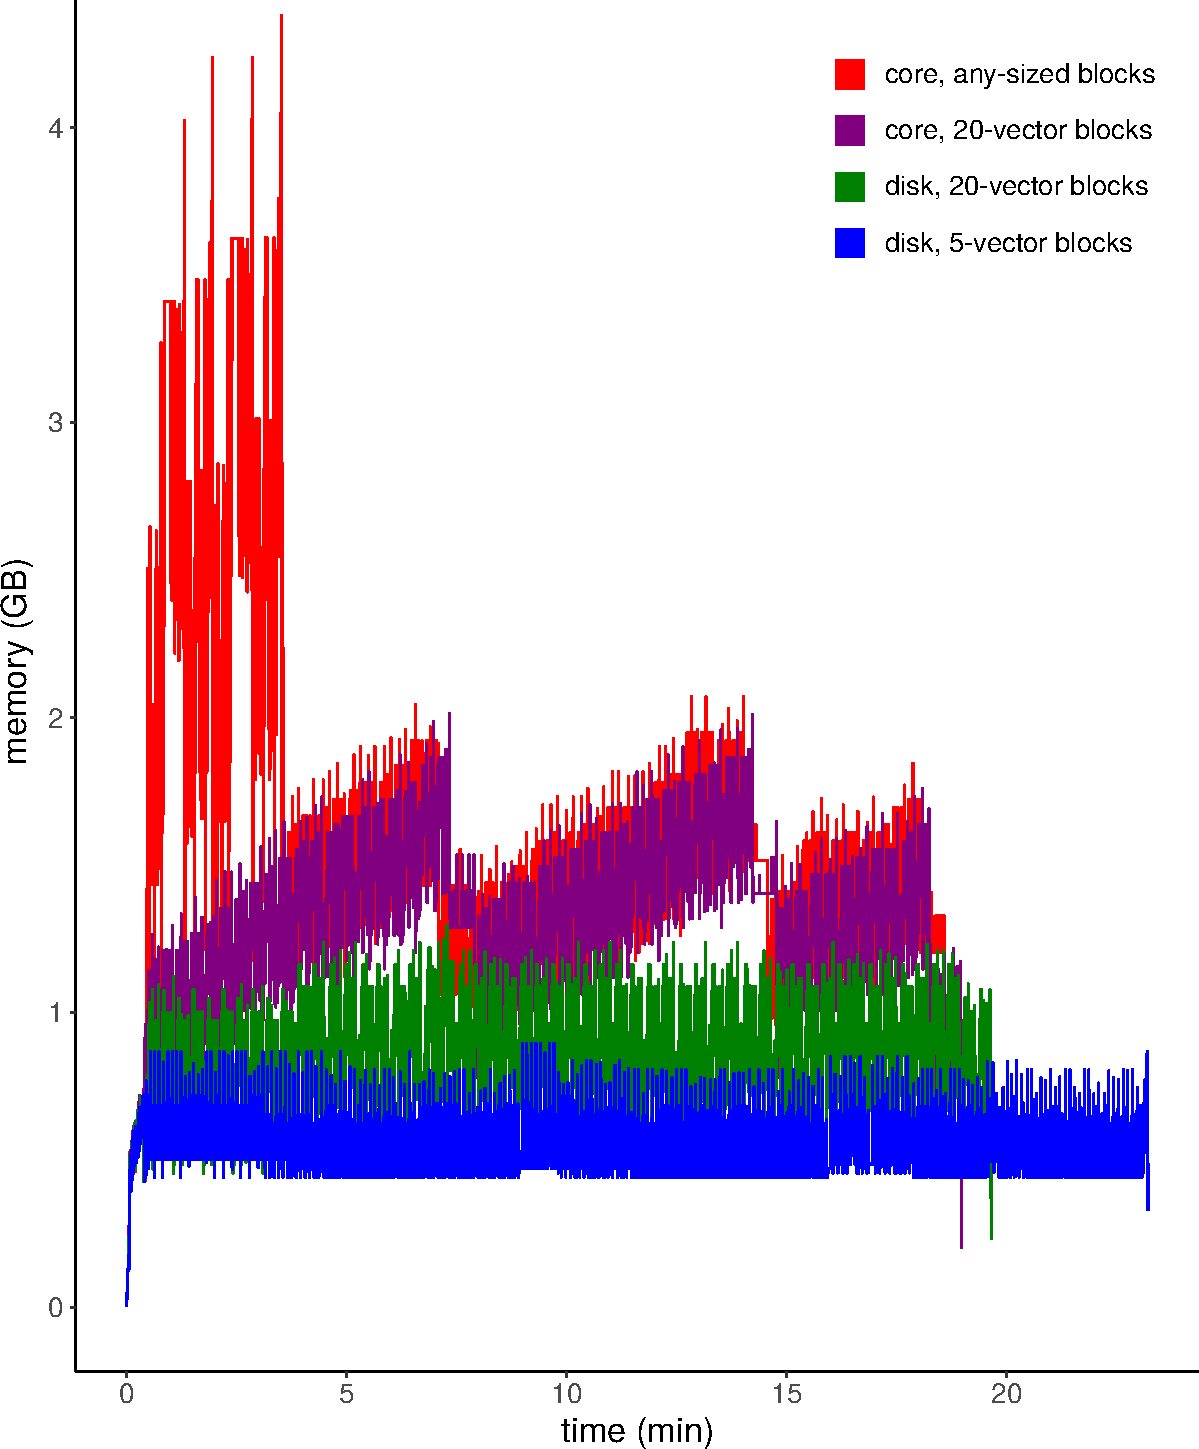
\includegraphics[width=\textwidth]{figures/mem_edited.pdf}
    \captionof{figure}{%
        LR-ODC-12 memory profiles for the lowest 20 states of ethylene with the
        def2-SV(P) basis set, computed on an
        Intel\textsuperscript{\textregistered} Core\texttrademark\ i7-5600U
        processor using four threads.
    }
}

\begin{enumerate}
    \item
        Note subspace collapses
\end{enumerate}


\begin{subappendices}
\section{LR-ODC-12 Linear Transformation Formulas}
\label{sec:linear-transformation-formulas}

\begin{equation}
    \begin{array}{r@{\,}l}
        (\mathbf{A}_{11}(\mathbf{u}_{\mu,1}))_{ia}
        =
        &
        h_j^i
        \gamma_a^b
        u_{\mu,b}^j
        +
        h_a^b
        \gamma_j^i
        u_{\mu,b}^j
        -
        (\bar{\mathbf{F}})_j^i
        u_{\mu,a}^j
        -
        (\bar{\mathbf{F}})_a^b
        u_{\mu,b}^i
        +
        \overline{g}_{nj}^{mi}
        \gamma_{ma}^{nb}
        u_{\mu,b}^j
        \\[5pt]
        &
        +
        \overline{g}_{ma}^{nb}
        \gamma_{nj}^{mi}
        u_{\mu,b}^j
        +
        \overline{g}_{jf}^{ie}
        \gamma_{ae}^{bf}
        u_{\mu,b}^j
        +
        \overline{g}_{ae}^{bf}
        \gamma_{jf}^{ie}
        u_{\mu,b}^j
        +
        \overline{g}_{me}^{ib}
        \gamma_{ja}^{me}
        u_{\mu,b}^j
        \\[5pt]
        &
        +
        \overline{g}_{ja}^{me}
        \gamma_{me}^{ib}
        u_{\mu,b}^j
    \end{array}
\end{equation}

\begin{equation}
    \begin{array}{r@{\,}l}
        (\mathbf{B}_{11}(\mathbf{u}_{\mu,1}))_{ia}
        =
        &
        \overline{g}_{be}^{im}
        \gamma_{ma}^{je}
        u_{\mu,j}^b
        +
        \overline{g}_{ma}^{je}
        \gamma_{be}^{im}
        u_{\mu,j}^b
        +
        \overline{g}_{mb}^{ie}
        \gamma_{ae}^{jm}
        u_{\mu,j}^b
        +
        \overline{g}_{ae}^{jm}
        \gamma_{mb}^{ie}
        u_{\mu,j}^b
        \\[5pt]
        &
        +
        \tfrac{1}{2}
        \overline{g}_{mn}^{ij}
        \gamma_{ab}^{mn}
        u_{\mu,j}^b
        +
        \tfrac{1}{2}
        \overline{g}_{ab}^{mn}
        \gamma_{mn}^{ij}
        u_{\mu,j}^b
        +
        \tfrac{1}{2}
        \overline{g}_{ef}^{ij}
        \gamma_{ab}^{ef}
        u_{\mu,j}^b
        +
        \tfrac{1}{2}
        \overline{g}_{ab}^{ef}
        \gamma_{ef}^{ij}
        u_{\mu,j}^b
    \end{array}
\end{equation}

\begin{equation}
    \begin{array}{r@{\,}l}
        (\mathbf{A}_{12}(\mathbf{u}_{\mu,2}))_{ia}
        =
        &
        -
        \tfrac{1}{2}
        \overline{g}_{la}^{cd}
        u_{\mu,cd}^{il}
        -
        \tfrac{1}{2}
        \overline{g}_{kl}^{id}
        u_{\mu,ad}^{kl}
        -
        \tfrac{1}{2}
        (\mathcal{I}_a^i)_k^m
        t_{ml}^{cd*}
        u_{\mu,cd}^{kl}
        -
        \tfrac{1}{2}
        (\mathcal{I}_a^i)_e^c
        t_{kl}^{ed*}
        u_{\mu,cd}^{kl}
        \\[5pt]
        &
        -
        \overline{g}_{ae}^{mc}
        t_{ml}^{ed*}
        u_{\mu,cd}^{il}
        -
        \overline{g}_{ke}^{im}
        t_{ml}^{ed*}
        u_{\mu,ad}^{kl}
        -
        \tfrac{1}{4}
        \overline{g}_{la}^{mn}
        t_{mn}^{cd*}
        u_{\mu,cd}^{il}
        \\[5pt]
        &
        -
        \tfrac{1}{4}
        \overline{g}_{ef}^{id}
        t_{kl}^{ef*}
        u_{\mu,ad}^{kl}
    \end{array}
\end{equation}

\begin{equation}
    \begin{array}{r@{\,}l}
        (\mathbf{B}_{12}(\mathbf{u}_{\mu,2}))_{ia}
        =
        &
        -
        \tfrac{1}{2}
        (\mathcal{I}_a^i)_m^k
        t_{cd}^{ml}
        u_{\mu,kl}^{cd}
        -
        \tfrac{1}{2}
        (\mathcal{I}_a^i)_c^e
        t_{ed}^{kl}
        u_{\mu,kl}^{cd}
        -
        \overline{g}_{ad}^{le}
        t_{ce}^{ki}
        u_{\mu,kl}^{cd}
        -
        \overline{g}_{md}^{il}
        t_{ca}^{km}
        u_{\mu,kl}^{cd}
        \\[5pt]
        &
        -
        \tfrac{1}{4}
        \overline{g}_{ma}^{kl}
        t_{cd}^{im}
        u_{\mu,kl}^{cd}
        -
        \tfrac{1}{4}
        \overline{g}_{cd}^{ie}
        t_{ae}^{kl}
        u_{\mu,kl}^{cd}
    \end{array}
\end{equation}

\begin{equation}
    \begin{array}{r@{\,}l}
        (\mathbf{A}_{21}(\mathbf{u}_{\mu,1}))_{ijab}
        =
        &
        -
        P^{(i/j)}
        \overline{g}_{ab}^{jc}
        u_{\mu,c}^i
        -
        P_{(a/b)}
        \overline{g}_{kb}^{ij}
        u_{\mu,a}^k
        -
        P^{(i/j)}
        (\mathcal{I}_k^c)_m^i
        t_{ab}^{mj}
        u_{\mu,c}^k
        \\[5pt]
        &
        -
        P_{(a/b)}
        (\mathcal{I}_k^c)_a^e
        t_{eb}^{ij}
        u_{\mu,c}^k
        -
        P_{(a/b)}^{(i/j)}
        \overline{g}_{ma}^{ce}
        t_{eb}^{mj}
        u_{\mu,c}^i
        -
        P_{(a/b)}^{(i/j)}
        \overline{g}_{km}^{ie}
        t_{eb}^{mj}
        u_{\mu,a}^k
        \\[5pt]
        &
        -
        \tfrac{1}{2}
        P^{(i/j)}
        \overline{g}_{mn}^{jc}
        t_{ab}^{mn}
        u_{\mu,c}^i
        -
        \tfrac{1}{2}
        P_{(a/b)}
        \overline{g}_{kb}^{ef}
        t_{ef}^{ij}
        u_{\mu,a}^k
    \end{array}
\end{equation}

\begin{equation}
    \begin{array}{r@{\,}l}
        (\mathbf{B}_{21}(\mathbf{u}_{\mu,1}))_{ijab}
        =
        &
        -
        P^{(i/j)}
        (\mathcal{I}_c^k)_m^i
        t_{ab}^{mj}
        u_{\mu,k}^c
        -
        P_{(a/b)}
        (\mathcal{I}_c^k)_a^e
        t_{eb}^{ij}
        u_{\mu,k}^c
        -
        P_{(a/b)}^{(i/j)}
        \overline{g}_{cb}^{je}
        t_{ae}^{ik}
        u_{\mu,k}^c
        \\[5pt]
        &
        -
        P_{(a/b)}^{(i/j)}
        \overline{g}_{kj}^{mb}
        t_{ac}^{im}
        u_{\mu,k}^c
        -
        \overline{g}_{mc}^{ij}
        t_{ab}^{km}
        u_{\mu,k}^c
        -
        \overline{g}_{ab}^{ke}
        t_{ce}^{ij}
        u_{\mu,k}^c
    \end{array}
\end{equation}

\begin{equation}
    \begin{array}{r@{\,}l}
        (\mathbf{A}_{22}(\mathbf{u}_{\mu,2}))_{ijab}
        =
        &
        -
        P_{(a/b)}
        \mathcal{F}_a^c
        u_{\mu,cb}^{ij}
        -
        P^{(i/j)}
        \mathcal{F}_k^i
        u_{\mu,ab}^{kj}
        +
        \tfrac{1}{2}
        \overline{g}_{ab}^{cd}
        u_{\mu,cd}^{ij}
        +
        \tfrac{1}{2}
        \overline{g}_{kl}^{ij}
        u_{\mu,ab}^{kl}
        \\[5pt]
        &
        -
        P_{(a/b)}^{(i/j)}
        \overline{g}_{la}^{jc}
        u_{\mu,cb}^{il}
        +
        \tfrac{1}{2}
        P_{(a/b)}
        \mathcal{G}_{af}^{ec}
        t_{eb}^{ij}
        t_{kl}^{fd*}
        u_{\mu,cd}^{kl}
        +
        \tfrac{1}{2}
        P_{(a/b)}
        \mathcal{G}_{ka}^{me}
        t_{eb}^{ij}
        t_{ml}^{cd*}
        u_{\mu,cd}^{kl}
        \\[5pt]
        &
        +
        \tfrac{1}{2}
        P^{(i/j)}
        \mathcal{G}_{me}^{ic}
        t_{ab}^{mj}
        t_{kl}^{ed*}
        u_{\mu,cd}^{kl}
        +
        \tfrac{1}{2}
        P^{(i/j)}
        \mathcal{G}_{mk}^{in}
        t_{ab}^{mj}
        t_{nl}^{cd*}
        u_{\mu,cd}^{kl}
    \end{array}
\end{equation}

\begin{equation}
    \begin{array}{r@{\,}l}
        (\mathbf{B}_{22}(\mathbf{u}_{\mu,2}))_{ijab}
        =
        &
        \tfrac{1}{2}
        P_{(a/b)}
        \mathcal{G}_{ac}^{ef}
        t_{eb}^{ij}
        t_{fd}^{kl}
        u_{\mu,kl}^{cd}
        +
        \tfrac{1}{2}
        P_{(a/b)}
        \mathcal{G}_{na}^{ke}
        t_{eb}^{ij}
        t_{cd}^{nl}
        u_{\mu,kl}^{cd}
        \\[5pt]
        &
        +
        \tfrac{1}{2}
        P^{(i/j)}
        \mathcal{G}_{mc}^{if}
        t_{ab}^{mj}
        t_{fd}^{kl}
        u_{\mu,kl}^{cd}
        +
        \tfrac{1}{2}
        P^{(i/j)}
        \mathcal{G}_{mn}^{ik}
        t_{ab}^{mj}
        t_{cd}^{nl}
        u_{\mu,kl}^{cd}
    \end{array}
\end{equation}

\begin{equation}
    (\mathbf{S}_{11}(\mathbf{u}_{\mu,1}))_{ia}
    =
    \gamma^i_j
    u_{\mu,a}^j
    -
    \gamma^b_a
    u_{\mu,b}^i
\end{equation}

\begin{equation}
    (\mathbf{S}_{11}^{-1}(\mathbf{u}_{\mu,1}))_{ia}
    =
    \frac{%
        (\mathbf{Y}^\dagger)_{j'}^i
        (\mathbf{Y})_a^{b'}
    }{%
        \gamma_{j'}-\gamma_{b'}
    }
    (\mathbf{Y}^\dagger)_{b'}^b
    (\mathbf{Y})_j^{j'}
    u_{\mu,b}^j
\end{equation}

\begin{equation}
    (\mathbf{Y}^\dagger)_{q'}^q
    \gamma_q^p
    (\mathbf{Y})_p^{p'}
    =
    \delta_{q'}^{p'}
    \gamma_{q'}
\end{equation}

\begin{equation}
    \begin{array}{r@{\,}l}
        (\tilde{\mathbf{A}}_{22})_{ijab,ijab}
        \equiv
        &
        -
        \mathcal{F}_i^i
        -
        \mathcal{F}_j^j
        -
        \mathcal{F}_a^a
        -
        \mathcal{F}_b^b
        +
        \overline{g}_{ij}^{ij}
        +
        \overline{g}_{ab}^{ab}
        -
        S(i/j|a/b)
        \overline{g}_{ia}^{ia}
        \\[10pt]
        &
        +
        S(a/b)
        \mathcal{G}_{af}^{ea}
        t_{eb}^{ij}
        t_{ij}^{fb}
        -
        S(a/b)
        \mathcal{G}_{af}^{eb}
        t_{eb}^{ij}
        t_{ij}^{fa}
        +
        2
        S(i/j|a/b)
        \mathcal{G}_{ia}^{me}
        t_{eb}^{ij}
        t_{mj}^{ab}
        \\[10pt]
        &
        +
        S(i/j)
        \mathcal{G}_{mi}^{in}
        t_{ab}^{mj}
        t_{nj}^{ab}
        -
        S(i/j)
        \mathcal{G}_{mj}^{jn}
        t_{ab}^{mi}
        t_{nj}^{ab}
    \end{array}
\end{equation}

\begin{equation}
    \begin{array}{r@{\,}l}
        (\tilde{\mathbf{B}}_{22})_{ijab,ijab}
        \equiv
        &
        +
        S(a/b)
        \mathcal{G}_{aa}^{ef}
        t_{eb}^{ij}
        t_{fb}^{ij}
        -
        S(a/b)
        \mathcal{G}_{ba}^{ef}
        t_{eb}^{ij}
        t_{fb}^{ij}
        +
        2
        S(i/j|a/b)
        \mathcal{G}_{ma}^{ia}
        t_{eb}^{ij}
        t_{ab}^{mj}
        \\[10pt]
        &
        +
        S(i/j)
        \mathcal{G}_{mn}^{ii}
        t_{ab}^{mj}
        t_{ab}^{nj}
        -
        S(i/j)
        \mathcal{G}_{mn}^{ij}
        t_{ab}^{mj}
        t_{ab}^{ni}
    \end{array}
\end{equation}

\end{subappendices}
